\chapter{散射、對偶性與 Veneziano 振幅}

\lectureoverview{散射將碰撞化約為可與實驗比較的不變量資料。對四個全同粒子而言，這些資料可用 Mandelstam 變數 \(s,t,u\) 表示，其中只有兩個彼此獨立。一般的粒子交換於是暗示存在不同的直接道與交叉道。Veneziano 振幅打破了這項預期：同一個函數包含兩種通道的描述。本講後半部將從兩條相接的開弦建構這個函數：兩弦接合後，成為一條振盪的弦鏈共同演化，之後再度分裂。}

\section{理論必須預測什麼}

費米弦解決了純玻色模型的兩項缺陷：它們容許費米子態，並且在適當投影後消除快子。它們的臨界時空維度是十，而非二十六。因此額外維度依然存在，只是緊緻化留待稍後討論。眼前的主題是散射。
\editorialnote{所謂無快子，指的是施加必要投影後得到的自洽超弦譜；單靠加入世界面費米子並不足以達成這點。}

散射未必是粒子最有趣的活動，只是實驗最容易一再重複的操作。讓指定的粒子彼此碰撞，記錄碰撞後出射的粒子，並由此推知相互作用區域內部的動力學。理論若要能作出定量預測，就必須給出一個複振幅
\begin{equation}
  \mathcal A(\hbox{incoming data}\to\hbox{outgoing data}),
\end{equation}
其絕對值平方再乘上通常的相空間因子，便得到該結果發生的機率。

\begin{figure}[H]
  \centering
  
\includegraphics[width=0.72\textwidth]{lecture_06_figure_01.png}
  \caption{入射粒子進入黑箱相互作用區域，出射粒子由其中離開；圖中以水平方向表示時間。}
  \lectureframe{00:02:35}
  \label{fig:l06-black-box}
\end{figure}

粒子也帶有自旋、電荷和種類等標記。為了先看清運動學，我們暫且不考慮動量以外的性質。

\section{四動量與全入射慣例}

將一個粒子的四動量寫成
\begin{equation}
  k^\mu=(k^0,\mathbf k)=(E,\mathbf p).
\end{equation}
本講採用 mostly-plus 度規，因此
\begin{equation}
  k^2\equiv \mathbf p^2-E^2.
\end{equation}
相對論色散關係於是為
\begin{equation}
  E^2-\mathbf p^2=m^2,
  \qquad
  k^2=-m^2.
  \label{eq:l06-mass-shell}
\end{equation}
改變空間動量會改變能量，但不會使粒子離開其質量殼。

\begin{figure}[H]
  \centering
  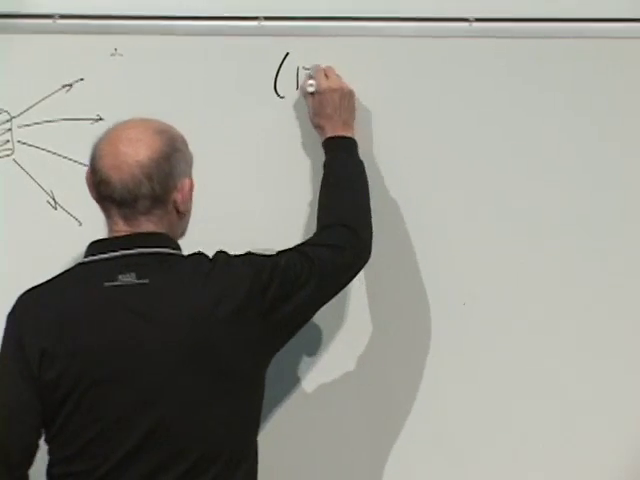
\includegraphics[width=0.66\textwidth]{lecture_06_figure_02.png}
  \caption{本講採用的度規慣例下，質量殼條件為何。}
  \lectureframe{00:05:56}
  \label{fig:l06-mass-shell}
\end{figure}

考慮兩個粒子以動量 \(k_1,k_2\) 入射，另有兩個粒子以物理動量 \(q_3,q_4\) 出射。能量與動量守恆可寫成一個四向量方程：
\begin{equation}
  k_1+k_2=q_3+q_4.
  \label{eq:l06-physical-conservation}
\end{equation}
方便的作法是把每條外線的動量都定義為入射動量：
\begin{equation}
  k_3\equiv-q_3,
  \qquad
  k_4\equiv-q_4.
\end{equation}
如此一來
\begin{equation}
  k_1+k_2+k_3+k_4=0,
  \label{eq:l06-all-incoming}
\end{equation}
而且每條外腿都滿足 \(k_i^2=-m_i^2\)。出射粒子只有在這套記帳慣例下才具有負能量；它們的物理能量仍為正。

\begin{figure}[H]
  \centering
  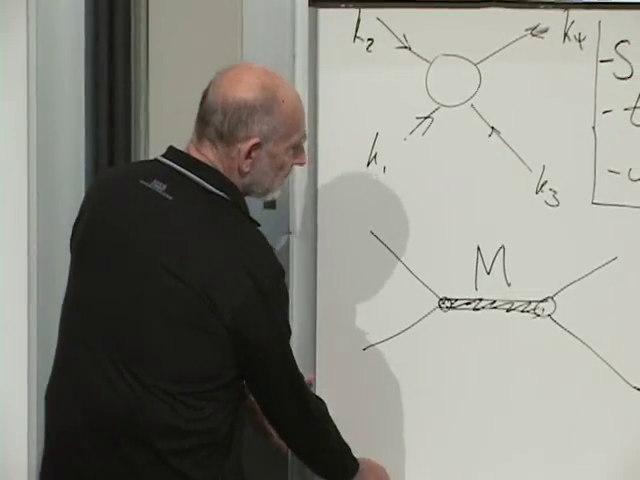
\includegraphics[width=0.68\textwidth]{lecture_06_figure_03.png}
  \caption{將物理出射動量反向，便可對稱地把四個外部動量全都視為入射。}
  \lectureframe{00:09:10}
  \label{fig:l06-all-incoming-board}
\end{figure}

乍看之下，振幅是十六個分量的函數，
\(\mathcal A(k_1,k_2,k_3,k_4)\)。其中大多數都是多餘的。轉到質心參考系，將入射動量旋轉至選定的軸上，並為求簡便，假設四個粒子的質量相同。如此一來，入射態便由一個數值決定，也就是質心能量。出射粒子的空間動量大小相等、方向相反，且大小與入射粒子對相同。剩下的只有偏轉角 \(\theta\)。因此，這個過程有兩個獨立的運動學變數：
\begin{equation}
  E_{\mathrm{cm}},
  \qquad
  \theta.
  \label{eq:l06-two-data}
\end{equation}

\section{Mandelstam 變數}

\eqref{eq:l06-two-data} 中的兩個物理量應能不依賴參考系地表示。採用全入射慣例，定義
\begin{equation}
  \begin{aligned}
    -s&=(k_1+k_2)^2,\\
    -t&=(k_1+k_3)^2,\\
    -u&=(k_1+k_4)^2.
  \end{aligned}
  \label{eq:l06-mandelstam}
\end{equation}
在質心參考系中，\(k_1+k_2\) 的空間部分彼此抵消，因此
\begin{equation}
  s=E_{\mathrm{cm}}^2.
  \label{eq:l06-s-energy}
\end{equation}

對出射粒子的物理動量 \(q_3=-k_3\)，
\begin{equation}
  k_1+k_3=k_1-q_3
\end{equation}
是由外腿 1 傳遞至外腿 3 的動量。若外部粒子的質量相同，且入射空間動量的大小為 \(p\)，則
\begin{equation}
  -t=2p^2(1-\cos\theta),
  \qquad
  -u=2p^2(1+\cos\theta).
  \label{eq:l06-tu-angle}
\end{equation}
因此，\(t\) 和 \(u\) 承載著探測器所測得的角度資訊。

\begin{figure}[H]
  \centering
  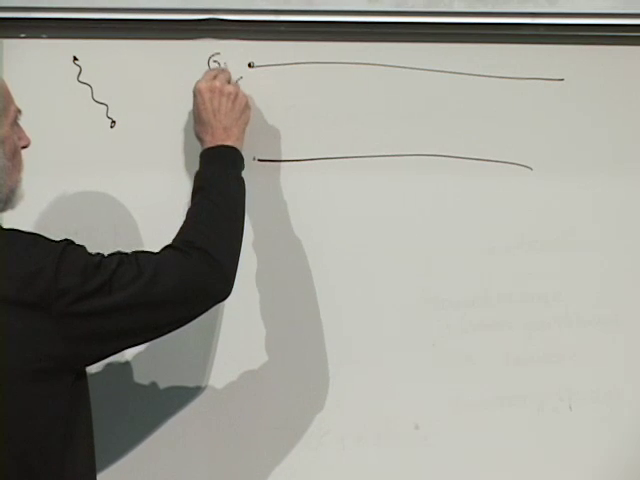
\includegraphics[width=0.74\textwidth]{lecture_06_figure_04.png}
  \caption{全入射慣例下 \(s,t,u\) 的對稱定義。}
  \lectureframe{00:26:20}
  \label{fig:l06-stu-board}
\end{figure}

三個符號不代表有三項獨立資料。將 \eqref{eq:l06-all-incoming} 平方並利用 \(k_i^2=-m^2\)，對等質量情況可得
\begin{equation}
  s+t+u=4m^2
  \label{eq:l06-stu-constraint}
\end{equation}
已知 \(s\) 與 \(t\) 後，\(u\) 便隨之確定。

\begin{classroomqa}
\audiencequestion{真空會像摩擦力一樣，使自由運動的粒子減速嗎？\lecturetimestamp{00:27:17}}
\lecturerresponse{在平移不變的真空中不會。動量不可能憑空消失，因此動量守恆禁止這種摩擦。可以設想某種介質，或另一種選定了優先靜止參考系的真空，但這裡討論的並非那種真空。}
\end{classroomqa}

\begin{classroomqa}
\audiencequestion{為什麼兩個出射粒子的能量必須相同？\lecturetimestamp{00:27:54}}
\lecturerresponse{在質心參考系中，兩者的空間動量必須大小相等、方向相反。對於這裡討論的等質量過程，動量大小相等，再由 \(E^2=p^2+m^2\) 可知能量也相等。若出射粒子的質量不同，這個結論就必須修正。}
\end{classroomqa}

\section{直接道與交叉道}

在一個簡單的點粒子圖中，粒子 1 和 2 形成質量為 \(M\) 的中間粒子，接著衰變成 3 和 4。略去分子因子及極點處方後，其典型依賴形式為
\begin{equation}
  \mathcal A_s\sim\frac{g^2}{s-M^2}.
  \label{eq:l06-s-channel}
\end{equation}
這是直接過程，也就是 \(s\) 道過程。將連結方式轉向一側，便得到兩條外線之間的交換：
\begin{equation}
  \mathcal A_t\sim\frac{g^2}{t-M^2},
  \label{eq:l06-t-channel}
\end{equation}
這是交叉過程，也就是 \(t\) 道過程。第三種連結方式則給出
\begin{equation}
  \mathcal A_u\sim\frac{g^2}{u-M^2}.
  \label{eq:l06-u-channel}
\end{equation}

\begin{figure}[H]
  \centering
  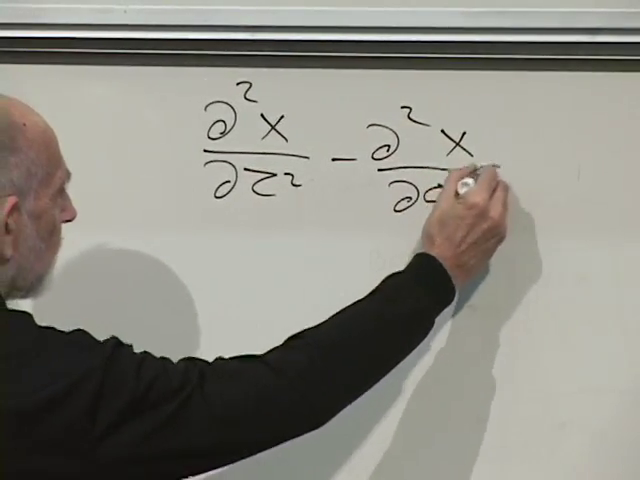
\includegraphics[width=0.72\textwidth]{lecture_06_figure_05.png}
  \caption{經由中間態直接生成，以及相應的極點 \(g^2/(s-M^2)\)；同一塊板上也正在拼出交叉道的連結方式。}
  \lectureframe{00:30:50}
  \label{fig:l06-channel-board}
\end{figure}

這項區別具有物理意義。在這個粗略的純量近似下，\eqref{eq:l06-s-channel} 取決於碰撞能量，而不取決於角度。複合態在衰變前已不再保留入射方向的資訊，因此衰變是各向同性的。交換振幅則取決於動量轉移，因而也取決於角度；交換粒子越輕，越傾向於小角度偏轉。自旋還會帶來額外的角度依賴，但極點結構在此已清楚可見。

\begin{classroomqa}
\audiencequestion{缺少的 \(u\) 道會不會產生第三項？\lecturetimestamp{00:34:47}}
\lecturerresponse{會，只要粒子的種類與耦合允許這種連結方式，就要加入在 \(u=M^2\) 有極點的一項。它不是新的獨立運動學變數，因為 \(s+t+u=4m^2\)；不過，它確實對應一種不同的道圖。}
\end{classroomqa}

\section{一個函數，兩種通道描述}

單一極點不足以描述介子散射。兩個介子可以形成許多共振態，具有一系列不同的質量與角動量。1960 年代初期，人們的第一個想法是加入更多 \(s\) 道極點、更多 \(t\) 道極點，以及所有允許的 \(u\) 道極點。後來，人們找到了一個精簡得多的函數。在本講採用的單位制中，線性 Regge 軌跡及其截距已吸收到 \(s\) 與 \(t\) 中，振幅為
\begin{equation}
  \mathcal A_{\mathrm V}(s,t)
  \propto
  \frac{\Gamma(-s)\Gamma(-t)}{\Gamma(-s-t)}.
  \label{eq:l06-veneziano}
\end{equation}
伽馬函數將階乘延伸為
\begin{equation}
  \Gamma(n)=(n-1)!
\end{equation}
此式在正整數處成立。

\begin{figure}[H]
  \centering
  \includegraphics[width=0.68\textwidth]{lecture_06_figure_06.png}
  \caption{以伽馬函數的對稱比值表示的 Veneziano 振幅。}
  \lectureframe{00:42:25}
  \label{fig:l06-veneziano-board}
\end{figure}

\(\Gamma(-s)\) 的極點重現了直接道共振態的無限序列。然而，同一個表示式在 \(s\leftrightarrow
t\) 下保持對稱，因此 \(\Gamma(-t)\) 的極點可展開成交叉道描述。這並非把兩項分別加入振幅；一個解析函數便容許兩種描述。這就是直接道共振態與交叉道交換之間的對偶性。

\begin{classroomqa}
\audiencequestion{一個振幅怎麼能同時包含兩個通道的求和，卻不把它們相加？\lecturetimestamp{00:43:32}}
\lecturerresponse{這正是令人驚訝之處。在 \(s\) 道極點附近展開這個函數，會得到直接道共振態的組織方式；在 \(t\) 道極點附近展開，則會以交換的方式呈現同一個函數。要說明這兩種解讀為何相同，必須有微觀模型，而這個模型就是相互作用的弦。}
\end{classroomqa}

\section{開弦掃出的一條帶狀面}

用下式參數化一條開弦：
\begin{equation}
  0\leq\sigma\leq\pi.
\end{equation}
標記 \(\sigma\) 並非時空位置。嵌入座標 \(X^\mu(\sigma,\tau)\) 描述這個帶標記的點在時空中的位置，而 \(\tau\) 則量度演化。點粒子掃出一條世界線；運動中的弦則掃出二維的世界面。在自由理論中，每個嵌入座標都滿足
\begin{equation}
  \frac{\partial^2X^\mu}{\partial\tau^2}
  -
  \frac{\partial^2X^\mu}{\partial\sigma^2}
  =0.
  \label{eq:l06-wave-equation}
\end{equation}

\begin{figure}[H]
  \centering
  \includegraphics[width=0.70\textwidth]{lecture_06_figure_07.png}
  \caption{描述世界面帶狀區域上各自由弦座標的波動方程。}
  \lectureframe{00:49:10}
  \label{fig:l06-wave-equation-board}
\end{figure}

建構散射過程時，最好不要太早取連續極限。將每條弦替換為 \(n\) 個以彈簧相連的質點。世界面便成為一系列密集分布、彼此鄰近的世界線，而其正規模態就是一般的諧振子。兩條入射弦鏈可以在端點處接觸；此時一根新彈簧將兩者接合，它們作為一條較長的弦鏈演化 \(\tau\)，之後彈簧斷開，兩條出射弦鏈便形成。

\begin{figure}[H]
  \centering
  \includegraphics[width=0.72\textwidth]{lecture_06_figure_08.png}
  \medskip

  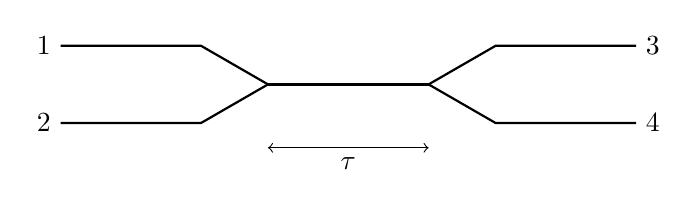
\begin{tikzpicture}[x=0.85cm,y=0.70cm]
    \draw[thick] (0,2.2) -- (2.1,2.2) -- (3.1,1.5);
    \draw[thick] (0,0.8) -- (2.1,0.8) -- (3.1,1.5);
    \draw[thick] (3.1,1.5) -- (5.5,1.5);
    \draw[thick] (5.5,1.5) -- (6.5,2.2) -- (8.6,2.2);
    \draw[thick] (5.5,1.5) -- (6.5,0.8) -- (8.6,0.8);
    \draw[<->] (3.1,0.35) -- node[below] {\(\tau\)} (5.5,0.35);
    \node[left] at (0,2.2) {1};
    \node[left] at (0,0.8) {2};
    \node[right] at (8.6,2.2) {3};
    \node[right] at (8.6,0.8) {4};
  \end{tikzpicture}
  \caption{兩條離散化的開弦相接，形成一條中間弦，持續 \(\tau\)，然後分裂。來源畫面保留了彈簧與世界線的構造；示意圖則凸顯其連結方式。}
  \lectureframe{00:51:25}
  \label{fig:l06-string-joining}
\end{figure}

圖中兩條弦只是在參數空間裡彼此相鄰。在端點座標實際重合之前，它們在時空中的位置不必相鄰。重參數化自由度讓我們可以把接合與分裂事件安排在圖中方便的位置；這項幾何自由度將在下一講轉化為共形對稱性。

\section{振子計算逐步拆解}

設第一條弦鏈的座標為 \(x_1,\ldots,x_n\)，第二條為 \(x_{n+1},\ldots,x_{2n}\)。它們的質心座標是
\begin{equation}
  X_{\mathrm{cm}}^{(1)}
  =\frac1n\sum_{a=1}^{n}x_a,
  \qquad
  X_{\mathrm{cm}}^{(2)}
  =\frac1n\sum_{a=n+1}^{2n}x_a.
  \label{eq:l06-chain-centers}
\end{equation}
動量確定為 \(k_1\) 的弦鏈，其波函數由質心平面波乘上內部振子的基態波函數構成：
\begin{align}
  \Psi_1
  &=
  e^{ik_1\cdot X_{\mathrm{cm}}^{(1)}}
  \psi_0(x_1,\ldots,x_n),
  \\
  \Psi_2
  &=
  e^{ik_2\cdot X_{\mathrm{cm}}^{(2)}}
  \psi_0(x_{n+1},\ldots,x_{2n}).
  \label{eq:l06-two-wavefunctions}
\end{align}
因子 \(\psi_0\) 只依賴相對座標，不受整條弦鏈共同平移影響。由於兩條入射弦起初是彼此分離的量子系統，
\begin{equation}
  \Psi_{\mathrm{in}}=\Psi_1\Psi_2.
  \label{eq:l06-product-state}
\end{equation}

\begin{figure}[H]
  \centering
  \includegraphics[width=0.76\textwidth]{lecture_06_figure_09.png}
  \caption{兩個動量平面波及各自的內部振子基態因子，以不同顏色表示。}
  \lectureframe{00:58:05}
  \label{fig:l06-wavefunctions-board}
\end{figure}

接合時，從這個波函數中選出兩個端點座標相等的部分：
\begin{equation}
  x_n=x_{n+1}.
  \label{eq:l06-endpoint-contact}
\end{equation}
此刻其餘座標保持不變。接著，所選出的態以單一較長弦鏈的哈密頓量 \(H_{\mathrm{joined}}\) 演化：
\begin{equation}
  \Psi(\tau)
  =
  e^{-iH_{\mathrm{joined}}\tau}\Psi(0).
  \label{eq:l06-time-evolution}
\end{equation}
最後，計算它與出射弦態乘積的重疊；這些出射態所帶的動量為 \(q_3,q_4\)。

\begin{figure}[H]
  \centering
  \includegraphics[width=0.76\textwidth]{lecture_06_figure_10.png}
  \caption{施加端點重合條件前的雙弦波函數。}
  \lectureframe{00:58:55}
  \label{fig:l06-endpoint-board}
\end{figure}

計算過程冗長，但並不神祕。每個內部座標都能分解為振子模態，因此接合時的重疊、時間演化與最後的投影，都可化為高斯振子的代數計算。尚未確定的只有接合後弦的存續時間 \(\tau\)。

\begin{classroomqa}
\audiencequestion{黑色和紅色的波函數要相加還是相乘？\lecturetimestamp{01:02:26}}
\lecturerresponse{相乘。兩個獨立系統的張量積態，在座標表象中以各自波函數的乘積表示。相加描述的是不同可能性間的疊加，而不是兩條入射弦同時存在。}
\end{classroomqa}

\begin{classroomqa}
\audiencequestion{為什麼要對中間時間 \(\tau\) 積分？\lecturetimestamp{01:04:04}}
\lecturerresponse{接合後的弦沒有固定的存續時間。依照費曼規則，必須對所有允許的歷史求振幅和。在這種描述中，剩下的連續歷史參數就是從接合到分裂之間的時間，因此求和便化為對 \(0\leq\tau<\infty\) 的積分。}
\end{classroomqa}

\section{從傳播時間到貝塔函數}

計算完振子重疊後，結果可整理為
\begin{equation}
  \mathcal A(s,t)
  \propto
  \int_0^\infty d\tau\,
  e^{\tau(s+1)}
  \bigl(1-e^{-\tau}\bigr)^{-t-1}
  e^{-\tau}.
  \label{eq:l06-tau-integral}
\end{equation}
最後的 \(e^{-\tau}\) 保留在式中，因為下一步的變數代換需要它作為雅可比因子。等價地，首尾兩個指數因子可合併為 \(e^{s\tau}\)。

\begin{figure}[H]
  \centering
  \includegraphics[width=0.76\textwidth]{lecture_06_figure_11.png}
  \caption{振子計算後的傳播時間積分式；獨立的 \(e^{-\tau}\) 因子提供變數代換所需的雅可比因子。}
  \lectureframe{01:06:45}
  \label{fig:l06-tau-integral-board}
\end{figure}

現在令
\begin{equation}
  z=e^{-\tau},
  \qquad
  dz=-e^{-\tau}\,d\tau.
  \label{eq:l06-z-substitution}
\end{equation}
當 \(\tau\) 從 \(0\) 增至 \(\infty\) 時，\(z\) 會從 \(1\) 降至 \(0\)。負號使積分上下限反轉，因此得到
\begin{equation}
  \mathcal A(s,t)
  \propto
  \int_0^1
  z^{-s-1}(1-z)^{-t-1}\,dz.
  \label{eq:l06-beta-integral}
\end{equation}

\begin{figure}[H]
  \centering
  \includegraphics[width=0.74\textwidth]{lecture_06_figure_12.png}
  \caption{代換 \(z=e^{-\tau}\) 顯示出尤拉貝塔積分的形式。}
  \lectureframe{01:08:49}
  \label{fig:l06-beta-integral-board}
\end{figure}

在端點收斂的範圍內，這個積分有直接定義；在其他範圍則以解析延拓定義。它就是尤拉貝塔函數：
\begin{equation}
  B(-s,-t)
  =
  \frac{\Gamma(-s)\Gamma(-t)}{\Gamma(-s-t)}.
  \label{eq:l06-beta-gamma}
\end{equation}

\begin{figure}[H]
  \centering
  \includegraphics[width=0.72\textwidth]{lecture_06_figure_13.png}
  \caption{黑板將變換後的積分辨認為 \(B(-s,-t)\)，並開始還原其伽馬函數形式。}
  \lectureframe{01:12:24}
  \label{fig:l06-beta-gamma-board}
\end{figure}

通道對稱性現在一目了然。在 \(z\mapsto1-z\) 下，
\begin{equation}
  \int_0^1 z^{-s-1}(1-z)^{-t-1}\,dz
  =
  \int_0^1 z^{-t-1}(1-z)^{-s-1}\,dz.
\end{equation}
因此 \(\mathcal A(s,t)=\mathcal A(t,s)\)。由兩條弦接合、之後再分裂所建構的過程，自然也包含交叉道的描述。
\editorialnote{本講在貝塔函數的引數中省略了 Regge 斜率與截距。標準記號會將 \(s,t\) 替換為相應的線性軌跡 \(\alpha(s),\alpha(t)\)。對偶性與變數代換的論證不受影響。}

\begin{classroomqa}
\audiencequestion{伽馬函數比值看起來像組合學中的階乘式。它是否有直接的物理計數詮釋？\lecturetimestamp{01:13:22}}
\lecturerresponse{在整數引數下，貝塔函數與例如 \(n!\,m!/(n+m)!\) 這樣的比值有關，但這裡並未主張存在某種組合機制。世界面積分也恰好會產生同一個特殊函數；不過，發現這個振幅的過程並非從這種類比出發。}
\end{classroomqa}

一個世界面之所以能以兩種通道來解讀，其背後尚未揭示的原因是共形對稱性。它允許像拉伸太妃糖一樣延展這個面，而不改變振幅，因而能將直接道中長時間的傳播區域轉換成交叉道的交換圖像。這項幾何解釋留待下一講討論。

\section{散射檢驗確立了什麼}
\enlargethispage{3\baselineskip}
\begingroup
\setlength{\medskipamount}{3pt plus 1pt minus 1pt}

離散弦鏈的接合圖像引出了最後一組問題。

\begin{classroomqa}
\audiencequestion{若兩條各由 \(n\) 個組成部分構成的弦鏈在端點接合，接合後是否會有 \(2n-1\) 個組成部分？這會改變費米子宇稱嗎？\lecturetimestamp{01:16:16}}
\lecturerresponse{在強子端點圖像中，相接觸的端點對可視為一對粒子與反粒子，兩者湮滅後，數目減少二，而非一。在連續極限下，\(2n\) 與 \(2n-2\) 之間的有限差異無關緊要；但費米子宇稱必須保持不變。格點上的組成部分只是連續弦的調節器，並非字面意義上的基本珠粒。}
\end{classroomqa}

\begin{classroomqa}
\audiencequestion{後續討論會深入介紹超弦的完整數學嗎？\lecturetimestamp{01:18:05}}
\lecturerresponse{只會用到其中選定的推論。接下來將討論世界面對稱性與緊緻化，之後再從另一個出發點切入：這個出發點於 1990 年代中期發展而成，也就是 M 理論。它的目標是從另一種觀點得到相同的物理；在這種觀點下，若干原本複雜的特徵會變得清晰。}
\end{classroomqa}

\begin{classroomqa}
\audiencequestion{這項接合規則只是從介子碰撞得到的線索嗎？\lecturetimestamp{01:20:02}}
\lecturerresponse{介子散射提供了歷史上的線索，但這項規則普遍適用於開弦。同樣的拓撲也描述開弦光子與其他開弦態的碰撞。兩條閉弦也會以類似方式接合與分裂，中間區域則是一條閉弦。}
\end{classroomqa}

\begin{classroomqa}
\audiencequestion{這項計算只適用於弦態為費米子的情況嗎？\lecturetimestamp{01:20:56}}
\lecturerresponse{不適用。最初的 Veneziano 計算描述的是玻色開弦。超弦需要額外的費米自由度，且被積函數的細節也會有所改變，但接合、傳播、投影與世界面對偶性的邏輯仍大致相同。}
\end{classroomqa}

在振子譜中找到自旋一或自旋二的態，固然令人振奮，卻還不足以證明其身分。它們的散射振幅提供了更有力的檢驗。光子振幅符合電荷守恆與規範不變性所要求的恆等式；引力子振幅則符合無質量自旋二場的相應限制。弦態在與有質量態及無質量態的交互作用中，以及彼此交互作用時，都通過了這些檢驗。因此，光子與引力子的稱呼是基於物理上的確認，而非僅憑極化態計數猜測。
\editorialnote{以現代術語來說，這些檢驗體現於非物理極化態的解耦、規範 Ward 恆等式，以及無質量自旋二態的普適低能耦合。}

\begin{classroomqa}
\audiencequestion{弦理論描述中的電荷本身從何而來？\lecturetimestamp{01:24:03}}
\lecturerresponse{講座結尾時，這個問題仍未解答。要回答它，必須先介紹弦理論的內部結構與端點結構；這些內容尚未談到，因此答案留待後續討論，而不屬於此處的散射推導。}
\end{classroomqa}
\endgroup
